% =============================================================================
% I. Introduction — topology as a learnable decision variable
% =============================================================================

\section{Introduction}
\label{sec:intro}

Existing multi-UAV cooperative policies typically assume that the
communication topology is predefined---a fixed radius neighborhood, a dense
graph, or a hand-crafted schedule---and then learn controllers on top of that
structure.
As swarm size grows, dense or fully open in-radius interaction increases
messaging intensity, injects redundant and noisy exchanges, and fails to
adapt when task needs change.
The core issue is therefore not merely that ``communication is expensive,''
but that \textbf{topology itself should be optimized jointly with task
execution}.

\paragraph{Limitation of prior pipelines.}
MAPPO-style CTDE stabilizes decentralized control~\cite{yu2022mappo}, and
graph guides (e.g., GAT) encode spatial relations for early coordination.
A common pipeline is
\begin{center}
policy $\;\rightarrow\;$ (predefined) communication $\;\rightarrow\;$ environment,
\end{center}
so agents cannot decide \emph{whether} an exchange is currently needed.
Random pruning or post-hoc message deletion can cut critical coordination
edges just as easily as redundant ones.

\paragraph{Our formulation.}
We treat interaction topology as a learnable decision variable:
\begin{center}
environment $\;\rightarrow\;$ learn communication topology $\;\rightarrow\;$ policy.
\end{center}
\begin{quote}
Unlike previous approaches that assume communication topology is predefined,
we formulate topology selection as a learnable optimization problem jointly
solved with cooperative decision-making.
\end{quote}
Concretely, AC-DSGF answers: \emph{when} to interact, \emph{with whom}, and
\emph{at what intensity} under a budget---i.e., adaptive topology learning
rather than communication reduction alone.

\paragraph{Method sketch.}
\textbf{AC-DSGF} (Adaptive Communication-Constrained Dynamic Sparse Graph
Fusion) learns a soft gate $g_{ij}^{t}$ on radius support, applies a Top-$K$
budget $A_t^{\mathrm{AC}}=A\odot E^{K}$, and optimizes
$\mathbb{E}[\sum r_t]-\lambda_c\mathbb{E}[\sum C_t]$, while residual guidance
$a=\pi(o)+\beta\Delta(\Phi)$ keeps communication assistive
(Fig.~\ref{fig:motivation}).

\begin{figure}[t]
  \centering
  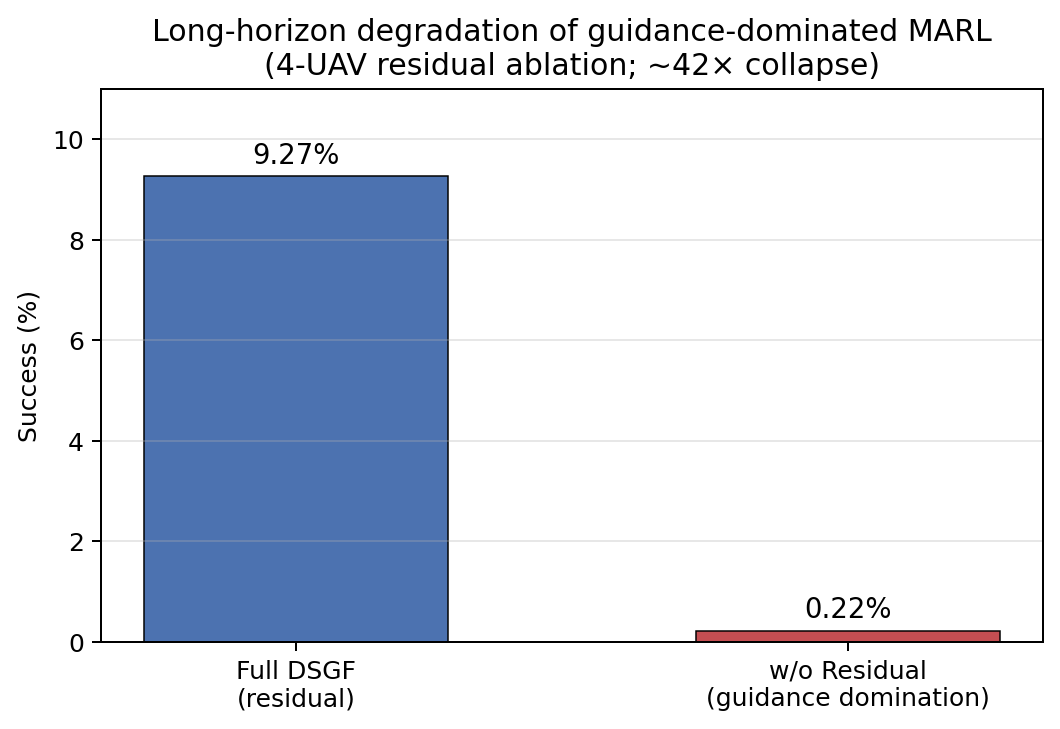
\includegraphics[width=0.78\linewidth]{figures/fig_motivation_degradation.png}
  \caption{Motivation: without residual decoupling, guided MARL can collapse
  under long-horizon optimization (4-UAV ablation; Table~\ref{tab:ablation}).
  AC-DSGF keeps residual guidance while learning budget-aware topology.}
  \label{fig:motivation}
\end{figure}

\paragraph{Claim.}
We position AC-DSGF as a mechanism for \textbf{learning scalable sparse
communication structure}, not as a Success maximizer.
Experiments show comparable task effectiveness with substantially lower Soft
Communication Activation Mass, density scaling $\eta_N=\mathcal{O}(K/N)$, and
deployable Top-$K$ discretization (Sec.~\ref{sec:scale-deploy}).

\paragraph{Contributions.}
\begin{enumerate}
  \item \textbf{Problem.}
        We formulate adaptive communication topology learning as a joint
        optimization problem between swarm performance and communication cost.
  \item \textbf{Method.}
        We propose a differentiable topology adaptation mechanism with budget
        regularization and residual guidance that jointly considers task
        relevance and communication budgets (Candidate Edge Scoring $\rightarrow$
        Budget-Constrained Edge Selection $\rightarrow$ Residual Recovery).
  \item \textbf{Validation.}
        We show comparable coordination performance with substantially lower
        Soft Communication Activation Mass (SCAM) under varying swarm scales
        and budgeted deployments.
\end{enumerate}
